% \begin{frame}{Anisotropy in stereotypical axon morphology}

%   %   
%   \begin{columns}
%     %     
%     \begin{column}{.425\textwidth}

%       %       \minipage[c][0.65\textheight][s]{\columnwidth}
%       \begin{figure}
%         \centering
%         \includegraphics<1>[width=0.85\textwidth]{%
%         figures/Romand2011_P14_1.png} %
%         \includegraphics<2>[width=0.9\textwidth]{%
%         figures/Romand2011_P14_2.png} 
%       \end{figure}
%       %       \endminipage

%     \end{column}
%     %     
%     \begin{column}{.575\textwidth}
%       \onslide<2->

%       %       \begin{figure}
%       %         \centering
%       %         \includegraphics[width=0.7\textwidth]{%
%       %         figures/Romand2011_P14_2.png} 
%       %       \end{figure}      


%     \end{column}
%   \end{columns}

%   \source{\cite{Romand2011}}
% \end{frame}


\begin{frame}{Anisotropy in stereotypical axon morphology}

  \only<1>{
    \begin{figure}
      \centering
      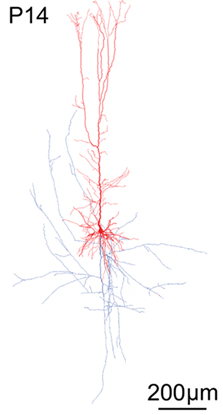
\includegraphics[height=0.75\textwidth]{%
        figures/Romand2011_P14_1.png} 
    \end{figure}}

  \only<2>{\vspace{0.5cm}
    \begin{figure}
      \centering
      \includegraphics[height=0.7\textwidth]{%
        figures/Romand2011_P14_2.png} 
    \end{figure}}

   \source{\only<1>{\cite{Romand2011}}\only<2>{\cite{Romand2011,Stepanyants2005}}}
  
\end{frame}
